
\documentclass[UTF8, onecolumn, a4paper]{article}
\usepackage{ctex}
\setlength{\parindent}{2em}
\usepackage{appendix}
\usepackage{geometry}
\usepackage{amsmath, amsthm}
\usepackage{multirow, multicol}
\usepackage{subfigure}
\usepackage{float}
\usepackage{graphicx}
\usepackage{lettrine}
\usepackage{authblk}
\usepackage{indentfirst}
\usepackage{xcolor, fontspec}%用于设置颜色
\usepackage[ruled,vlined]{algorithm2e}
\usepackage{listings}%用于显示代码
\usepackage[colorlinks,
linkcolor=red,
anchorcolor=blue,
citecolor=green
]{hyperref}
\usepackage{tikz}
\usetikzlibrary{trees}
\geometry{left=3.0cm,right=3.0cm,top=2.0cm,bottom=2.0cm}


\title{\textbf{高性能计算导论: Homework 3}}%———总标题
\author{刘泓尊\quad 2018011446\quad 计84}
%\affil{Department of Computer Science, Tsinghua University}

\begin{document}
\maketitle
\tableofcontents
\lstset{%代码块全局设置
	backgroundcolor=\color{red!3!green!3!blue!3},%代码块背景色为浅灰色
	rulesepcolor= \color{gray}, %代码块边框颜色
	breaklines=true,  %代码过长则换行
	numbers=left, %行号在左侧显示
	numberstyle= \small,%行号字体
	%keywordstyle= \color{red},%关键字颜色
	commentstyle=\color{gray}, %注释颜色
	frame=shadowbox,%用方框框住代码块
	xleftmargin=1em,
	xrightmargin=0em,
	tabsize=5,
	%rulesepcolor=\color{red!20!green!20!blue!20},  %阴影颜色
	keywordstyle={\color{blue!90!}\fontspec{Consolas Bold}},   %关键字颜色
	commentstyle={\color{blue!70!black}\fontspec{Consolas Italic}},   %注释颜色
	stringstyle=\color{orange!100!black}, %字符串颜色
	numberstyle=\color{purple}, %行号颜色
	%basicstyle=\ttfamily, %代码风格
	basicstyle=\fontspec{Consolas},
	showstringspaces=false,          % underline spaces within strings only  
	showtabs=false,
	captionpos=t, %文件标题位置
	flexiblecolumns
}

\section{File Structure}
\tikzstyle{every node}=[draw=black,thick,anchor=west]
\tikzstyle{selected}=[draw=red,fill=red!30]
\tikzstyle{optional}=[dashed,fill=gray!50]
\begin{center}
\begin{tikzpicture}
[
grow via three points={one child at (0.5,-0.7) and
	two children at (0.5,-0.7) and (0.5,-1.4)},
edge from parent path={(\tikzparentnode.south)  |-(\tikzchildnode.west)}]
\node {2018011446}
child { node {prog3\_1}
	child {node {Makefile}}
	child {node {prog3\_1\_histo\_dist.c}}
}
child [missing] {}				
child [missing] {}
child { node {prog3\_5}
	child {node {Makefile}}
	child {node {prog3\_5.cpp}}
}
child [missing] {}				
child [missing] {}
child { node {prog3\_6}
	child {node {Makefile}}
	child {node {prog3\_6.cpp}}
}
child [missing] {}				
child [missing] {}
child { node {prog3\_11}
	child {node {Makefile}}
	child {node {mpi\_prefix\_sum.c}}
}
child [missing] {}				
child [missing] {}
child { node {prog3\_13}
	child {node {Makefile}}
	child {node {mpi\_vector\_add.c}}
}
child [missing] {}				
child [missing] {}
child { node {2018011446\_刘泓尊\_hw3.pdf}};
\end{tikzpicture}
\end{center}


\section{Exercise 3.13}
\subsection{运行方式}
\subparagraph*{}
./prog3\_13下放有makefile,在该目录下执行“\textbf{make}”可以得到可执行程序; 之后执行“\textbf{make run p=...}”可以运行程序。其中p的值可以任选,如“\textbf{make run p=10}”; 运行程序后,会有提示进一步输入n; 执行“\textbf{make clean}”可以删除生成的.o文件和可执行程序。
\subparagraph*{}
在本程序中,为了测试更普适的条件,我将两个向量设为程序\textbf{随机生成},而不是从stdin读入。
\subsection{代码思路}
\paragraph*{}
为了实现n可以不被p整除的情况,我使用MPI\_Scatterv()和MPI\_Gatherv()函数实现向量元素的分发与收集。这两个函数需要显式指定每个进程得到的元素个数$count$和相对原向量的偏移量$disp$。
\paragraph*{}
为了实现数据比较均匀的分配,我使用作业1中一个题目的做法,先为每个进程分配$n/p$个元素,之后再将$n - (n/p)\cdot p$个元素给前$n - (n/p)\cdot p$个进程各一个。并以此为依据构建$disp$偏移量。
\paragraph*{}
具体代码如下:
\begin{lstlisting}[language={c}, title={Allocate\_count\_disp()}] 
int overflow = n - (n / comm_sz) * comm_sz;
int base = n / comm_sz;
for(i = 0; i < comm_sz; i++){
	(*count)[i] = base;
}
for(i = 0; i < overflow; i++){
	(*count)[i] += 1;
}
for((*disp)[0] = 0, i = 1; i < comm_sz; i++){
	(*disp)[i] = (*disp)[i-1] + (*count)[i-1];
}
\end{lstlisting}
\begin{lstlisting}[language={c}, title={Read\_vector()}] 
MPI_Scatterv(a, count, disp, MPI_DOUBLE, local_a, count[my_rank], MPI_DOUBLE, 0, comm);
\end{lstlisting}
\begin{lstlisting}[language={c}, title={Print\_vector()}] 
MPI_Gatherv(local_b, count[my_rank], MPI_DOUBLE, b, count, disp, MPI_DOUBLE, 0, comm);
\end{lstlisting}
\subsection{测试结果}
下例给出了$p=4,n=15$时的运行结果。可以看到,程序实现了在$n$不被$p$整除的情况下的向量加法。二范数误差$error<1e^{-6}$.
\begin{lstlisting}[language={}]
[2018011446@bootstraper prog3_13]$ make run p=4
srun -n 4 -l ./vectoradd
0: What's the order of the vectors?
15
0: x is
0: 0.887164 0.060926 0.839742 -0.539429 -0.333756 -0.310390 0.007394 -0.574869 0.205154 0.839252 -0.208210 0.947841 0.851419 0.031242 0.545745 
0: y is
0: -0.343533 -0.527309 -0.899562 0.181500 0.743957 0.918453 0.086991 -0.257361 -0.569818 -0.679560 0.243786 -0.304110 0.199846 -0.652993 0.659348 
0: The sum is
0: 0.543631 -0.466383 -0.059820 -0.357929 0.410201 0.608063 0.094386 -0.832231 -0.364665 0.159691 0.035576 0.643730 1.051265 -0.621751 1.205093 
\end{lstlisting}

\section{Exercise 3.11(d)}
\subsection{运行方式}
\subparagraph*{}
./prog3\_11下放有makefile,在该目录下执行“\textbf{make}”可以得到可执行程序; 之后执行“\textbf{make run p=...}”可以运行程序。其中p的值可以任选,如“\textbf{make run p=10}”(默认p=4); 执行“\textbf{make clean}”可以删除生成的.o文件和可执行程序;
\subparagraph*{}
为了便于检验程序正确性,在debug模式下可以输出每个进程产生的数组元素。即执行“\textbf{make debug}”产生调试模式下的可执行程序,再执行“\textbf{make run p=...}”可以观察输出。
\subparagraph*{}
运行程序后,每个进程会随机生成10个元素的数组,数值范围$[0,10)$$\footnote{进程内随机数的生成加了pid的偏移srand(pid+time(NULL));}$,最终在主进程中输出总共$10p$个元素数组的前缀和。
\subsection{代码思路}
首先在每个进程内计算数组的前缀和,保存在local\_prefix\_sum[]中。
\begin{lstlisting}[language={c}] 
//compute local prefix sum of local_a
local_prefix_sum[0] = local_a[0];
for(i = 1; i < LOCAL_N; i++){
	local_prefix_sum[i] = local_prefix_sum[i-1] + local_a[i];
}
\end{lstlisting}
之后使用MPI\_Scan()函数得到在该进程编号之前的所有进程数组的和(pred).
\begin{lstlisting}[language={c}] 
//Perform MPI_Scan() get pred_sum, (local sum == local_prefix_sum[LOCAL_N])
MPI_Scan(&local_prefix_sum[LOCAL_N-1], &pred, 1, MPI_INT, MPI_SUM, MPI_COMM_WORLD);
pred -= local_prefix_sum[LOCAL_N-1];
\end{lstlisting}
之后为每个进程内的local\_prefix\_sum[]都加上pred,此时的local\_prefix\_sum[]便是在全部进程的大数组中的前缀和。
\begin{lstlisting}[language={c}] 
//add pred sum
for(i = 0; i < LOCAL_N; i++){
	local_prefix_sum[i] += pred;
}
\end{lstlisting}
最后调用MPI\_Gather()收集到主进程输出.
\subsection{测试结果}
下列样例执行了“make run p=4”命令,程序在每个线程中生成10个元素,共40个元素.
\par 在debug模式下可以看到,程序正确地输出了前缀和。
\begin{lstlisting}[language={}, title={debug模式}]
[2018011446@bootstraper prog3_11]$ make run
srun -n 4 -l ./prefixsum
0: Process 0, vec:
0: 4 7 0 8 3 1 0 9 8 6 
1: Process 1, vec:
1: 5 1 7 4 3 1 3 4 0 3 
2: Process 2, vec:
2: 6 9 8 7 3 0 2 9 4 0 
3: Process 3, vec:
3: 7 6 2 4 5 1 3 7 7 9 
0: Prefix sum:
0: 4 11 11 19 22 23 23 32 40 46 51 52 59 63 66 67 70 74 74 77 83 92 100 107 110 110 112 121 125 125 132 138 140 144 149 150 153 160 167 176  
\end{lstlisting}
\begin{lstlisting}[language={}, title={release模式}]
[2018011446@bootstraper prog3_11]$ make run p=4
srun -n 4 -l ./prefixsum
0: Prefix sum:
0: 7 12 20 20 24 32 40 42 49 54 56 56 60 63 63 66 71 77 78 80 82 82 87 96 101 109 114 115 122 126 126 127 132 140 147 150 150 152 158 160 
\end{lstlisting}



\section{Exercise 3.1}
\subsection{运行方式}
\subparagraph*{}
./prog3\_1下放有makefile,在该目录下执行“\textbf{make}”可以得到可执行程序; 之后执行“\textbf{make run p=...}”可以运行程序。其中p的值可以任选,如“\textbf{make run p=10}”(默认p=4); 执行“\textbf{make clean}”可以删除生成的.o文件和可执行程序;
\subparagraph*{}
运行程序后,根据提示分别输入桶的个数$bins$、最小值$min$和最大值$max$,数据个数$n$。注意,$n$应能被$p$整除。
\subsection{代码思路}
代码完善了Find\_bins()和Which\_bin()函数。
\subparagraph*{Which\_bin():}考虑到桶的个数不是很多(通常$<1000$ ),所以采用线性查找其实可以很快的得到结果。将$data$与桶的边界依次比较即可。如果桶的数量$>10000$,可以将线性查找改为二分查找,以达到更快的搜索速度。
\begin{lstlisting}[language={c}, title={Which\_bin()}]
int Which_bin(float data, float bin_maxes[], int bin_count, float min_meas) {
	if(min_meas <= data && data <= bin_maxes[0]){
		return 0;
	} else {//bin_maxes[] bounds are [left, right);
		int i;
		for(i = 1; i < bin_count; i++){
			if (bin_maxes[i-1] <= data && data < bin_maxes[i]){
				return i;
			}
		}
		return bin_count - 1;
	}
} /* Which_bin */
\end{lstlisting}
\subparagraph*{Find\_bins():}
对当前进程的每个元素$data$,找到$data$所属的桶之后,将loc\_bin\_cts[]对应的桶编号位置+1即可。在本进程所有元素都统计完毕后,使用MPI\_Reduce()函数将所有的loc\_bin\_cts[]进行加总,存入bin\_counts[]中。
\begin{lstlisting}[language={c}, title={Find\_bins()}]
void Find_bins(int bin_counts[], float local_data[],int loc_bin_cts[], int local_data_count, float bin_maxes[], int bin_count, float min_meas, MPI_Comm comm){
	/* Use a for loop to find bins, the statement in the loop can be:
	bin = Which_bin(local_data[i], bin_maxes, bin_count, min_meas);
	Then, calculate the global sum using collective communication.
	*/
	int i;
	for(i = 0; i < local_data_count; i++){
		loc_bin_cts[Which_bin(local_data[i], bin_maxes, bin_count, min_meas)] ++;
	}
	MPI_Reduce(loc_bin_cts, bin_counts, bin_count, MPI_INT, MPI_SUM, 0, comm);
}  /* Find_bins */
\end{lstlisting}
\subsection{测试结果}
下列样例给出了执行“make run p=4”且$n=100, bin=5, min=0, max=100$的运行结果。
\begin{lstlisting}[language={}, title={$p=4, n=100, bin=5, min=0, max=100$}]
[2018011446@bootstraper prog3_1]$ make run p=4
srun -n 4 -l ./histodist
0: Enter the number of bins
5
0: Enter the minimum measurement
0
0: Enter the maximum measurement
100
0: Enter the number of data
100
0: 0.000-20.000:        XXXXXXXXXXXXXXX
0: 20.000-40.000:       XXXXXXXXXXXXXXXXXXXX
0: 40.000-60.000:       XXXXXXXXXXXXXXXXXX
0: 60.000-80.000:       XXXXXXXXXXXXXXXXXXXXX
0: 80.000-100.000:      XXXXXXXXXXXXXXXXXXXXXXXXXX
\end{lstlisting}



\section{Exercise 3.5}
\subsection{运行方式}
\subparagraph*{}
./prog3\_5下放有makefile,在该目录下执行“\textbf{make}”可以得到可执行程序; 之后执行“\textbf{make run p=... n=...}”可以运行程序。其中p的值可以任选,如“\textbf{make run p=10 n=1000}”(默认p=4, n=12); 执行“\textbf{make clean}”可以删除生成的.o文件和可执行程序; 注意: n应能被p整除。
\subparagraph*{}
运行程序后,程序会随机生成一个$n\times n$的$double$矩阵和$n$维随机向量,分别采用按列分块的并行和串行策略计算$y = Ax$,统计并输出串行/并行运行时间、加速比、二范数误差等结果。
\subsection{代码思路}
\paragraph*{run\_col():}
\subparagraph*{}
为了使得数据可以按列分块进行数据分发,本函数创建了派生数据类型col\_t,表示按列分块的矩阵.
\par 将矩阵$matrix$按列分块为$p$个$n \times \frac{n}{p}$的竖长形矩阵$A_{i,(n\times local\_n)}$,使用MPI\_Scatter()函数分配到每个进程.
\par 将$vector$均分为$p$个$\frac{n}{p}$维的向量$loc\_vec$,使用MPI\_Scatter()函数分配到每个进程;
\par 之后在进程内计算结果$loc\_res = A_{i,(n\times local\_n)}\cdot loc\_vec$,是一个$n$维向量。
\par 最后使用MPI\_Reduce()函数加总各个进程的结果即可。
\begin{lstlisting}[language={c++}, title={创建派生数据类型}]
int local_n = n / comm_sz;
MPI_Datatype vec_t, col_t;
MPI_Type_vector(n, local_n, n, MPI_DOUBLE, &vec_t);
MPI_Type_create_resized(vec_t, 0, local_n * sizeof(double), &col_t);
\end{lstlisting}
\begin{lstlisting}[language={c++}, title={数据分发与收集}]
//Scatter data
MPI_Scatter(matrix, 1, col_t, loc_A, n * local_n, MPI_DOUBLE, 0, comm);
MPI_Scatter(vector, local_n, MPI_DOUBLE, loc_vec, local_n, MPI_DOUBLE, 0, comm);
//Reduce data
MPI_Reduce(loc_res, result, n, MPI_DOUBLE, MPI_SUM, 0, comm);
\end{lstlisting}
\begin{lstlisting}[language={c++}, title={计算}]
for(int i = 0; i < n; i++){
	loc_res[i] = 0.0;
	for(int j = 0; j < local_n; j++){
		loc_res[i] += loc_A[i * local_n + j] * loc_vec[j];
	}
}
\end{lstlisting}
\subsection{测试结果}
下列样例运行“make run p=4 n=100”得到如下结果,可以看到,本例并行算法的二范数误差$error < 1e^{-10}$,达到了预期要求:
\begin{lstlisting}[language={}, title={$p=4, n=100$}]
[2018011446@bootstraper prog3_5]$ make run p=4 n=100
srun -n 4 -l ./matvectmul 100
0: error(2 norm):                                 0.00000000000001238903
0: time (Serial)                                  0.000023s 
0: time (with MPI_Scatter/MPI_Reduce)             0.000660s 
0: time (without MPI_Scatter/MPI_Reduce)          0.000005s 
0: time (Scatter&Reduce)                          0.000655s 
0: Speedup ratio(with MPI_Scatter/MPI_Reduce)     0.0345 
0: Speedup ratio(without MPI_Scatter/MPI_Reduce)  4.5651
\end{lstlisting}
\subsection{性能评估}
下表展示了不同进程数$p$和矩阵大小$n$的性能测试结果:\\
运行时间及加速比的统计表与统计图如下:
\begin{table}[htb]
	\centering
	\begin{tabular}{l|lllllll}
		\hline
		$n \backslash p$& 1 & 2 & 4 & 8 & 10 & 16 & 20 \\ \hline
		2000 & 0.017 & 0.021 & 0.020 & 0.017 & 0.006 & 0.017 & 0.051 \\ \hline
		5000 & 0.090 & 0.115 & 0.117 & 0.099 & 0.094 & \#N/A & 0.092 \\ \hline
		10000 & 0.348 & 0.443 & 0.461 & 0.476 & 0.467 & 0.451 & 0.049 \\ \hline
		16000 & 0.820 & 1.001 & 1.044 & 1.037 & 1.041 & 1.747 & 1.077 \\ \hline
		20000 & 1.389 & 1.778 & 1.841 & 1.849 & 1.813 & 3.960 & 2.171 \\ \hline
		30000 & 3.287 & 4.087 & 4.193 & 4.106 & 4.058 & 3.982 & 4.421 \\ \hline
	\end{tabular}
	\caption{Total time (s)}
\end{table}
\begin{table}[htb]
	\centering
	\begin{tabular}{l|lllllll}
		\hline
		$n \backslash p$& 1 & 2 & 4 & 8 & 10 & 16 & 20 \\ \hline
		2000 & 0.005 & 0.003 & 0.001 & 0.001 & 0.0008 & 0.0003 & 0.0002 \\ \hline
		5000 & 0.028 & 0.014 & 0.007 & 0.003 & 0.003 & \#N/A & 0.002 \\ \hline
		10000 & 0.102 & 0.051 & 0.028 & 0.015 & 0.012 & 0.008 & 0.024 \\ \hline
		16000 & 0.255 & 0.116 & 0.065 & 0.034 & 0.028 & 0.032 & 0.027 \\ \hline
		20000 & 0.415 & 0.206 & 0.117 & 0.091 & 0.051 & 0.071 & 0.050 \\ \hline
		30000 & 1.034 & 0.516 & 0.262 & 0.134 & 0.114 & 0.081 & 0.110 \\ \hline
	\end{tabular}
	\caption{Compute time (s)}
\end{table}
\begin{table}[htb]
	\centering
	\begin{tabular}{l|lllllll}
		\hline
		$n \backslash p$& 1 & 2 & 4 & 8 & 10 & 16 & 20 \\ \hline
		2000 & 0.011 & 0.018 & 0.018 & 0.016 & 0.018 & 0.016 & 0.051 \\ \hline
		5000 & 0.063 & 0.101 & 0.11 & 0.095 & 0.09 & \#N/A & 0.090 \\ \hline
		10000 & 0.245 & 0.392 & 0.433 & 0.461 & 0.454 & 0.443 & 0.471 \\ \hline
		16000 & 0.564 & 0.886 & 0.979 & 1.004 & 1.012 & 1.716 & 1.050 \\ \hline
		20000 & 0.974 & 1.572 & 1.724 & 1.758 & 1.762 & 3.889 & 2.121 \\ \hline
		30000 & 2.253 & 3.569 & 3.931 & 3.973 & 3.944 & 3.901 & 4.303 \\ \hline
	\end{tabular}
	\caption{Communication time (s)}
\end{table}
\begin{table}[htb]
	\centering
	\begin{tabular}{l|lllllll}
		\hline
		$n \backslash p$& 1 & 2 & 4 & 8 & 10 & 16 & 20 \\ \hline
		2000 & 0.3581 & 0.2806 & 0.3183 & 0.3476 & 0.2446 & 0.3506 & 0.3767 \\ \hline
		5000 & 0.296 & 0.2372 & 0.2273 & 0.2776 & 0.2428 & \#N/A & 0.297 \\ \hline
		10000 & 0.2823 & 0.2179 & 0.2317 & 0.2303 & 0.2375 & 0.2426 & 0.2214 \\ \hline
		16000 & 0.2848 & 0.2175 & 0.2365 & 0.2331 & 0.2346 & 0.2501 & 0.2301 \\ \hline
		20000 & 0.2837 & 0.2216 & 0.2392 & 0.238 & 0.2937 & 0.2519 & 0.2036 \\ \hline
		30000 & 0.2866 & 0.2432 & 0.2375 & 0.2422 & 0.3391 & 0.2510 & 0.2576 \\ \hline
	\end{tabular}
	\caption{Speedup Ratio(考虑数据分发)}
\end{table}
\begin{table}[htb]
	\centering
	\begin{tabular}{l|lllllll}
		\hline
		& 1 & 2 & 4 & 8 & 10 & 16 & 20 \\ \hline
		2000 & 1.0415 & 2.0932 & 4.1795 & 7.8404 & 7.7315 & 15.4281 & 16.0935 \\ \hline
		5000 & 0.9676 & 1.9125 & 3.7297 & 6.9176 & 8.4419 & \#N/A & 12.9149 \\ \hline
		10000 & 0.956 & 1.8704 & 3.7659 & 7.2619 & 8.5391 & 10.6438 & 9.5133 \\ \hline
		16000 & 0.9656 & 1.8797 & 3.7799 & 7.2342 & 8.6007 & 10.6960 & 9.0774 \\ \hline
		20000 & 0.953 & 1.9125 & 3.7644 & 7.3127 & 8.597 & 10.9949 & 8.7999 \\ \hline
		30000 & 0.9668 & 1.9237 & 3.8066 & 7.4312 & 8.6962 & 10.9626 & 9.6352 \\ \hline
	\end{tabular}
	\caption{Speedup Ratio(不考虑数据分发)}
\end{table}
\begin{figure}[htb]
	\centering
	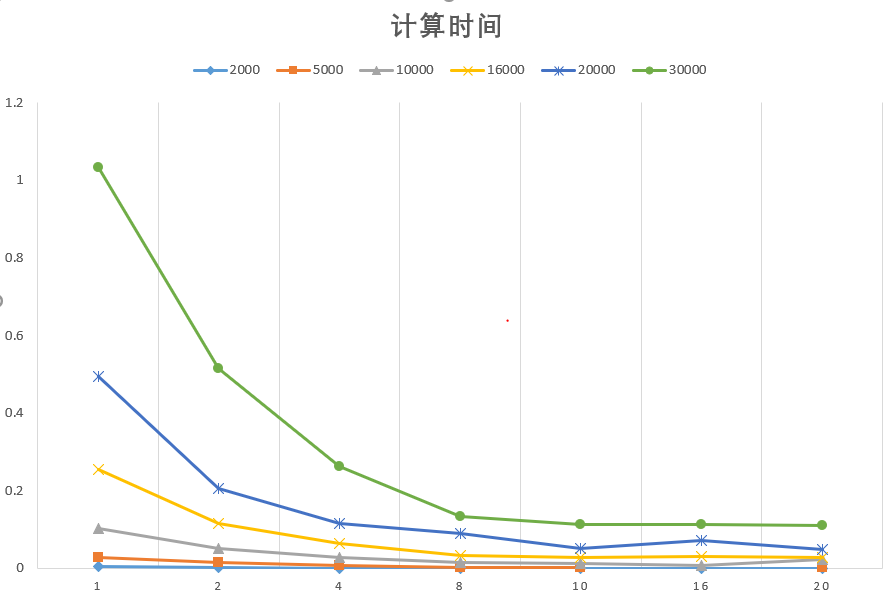
\includegraphics[width=0.8\textwidth]{hw3_5.png}
\end{figure}
\begin{figure}[htb]
	\centering
	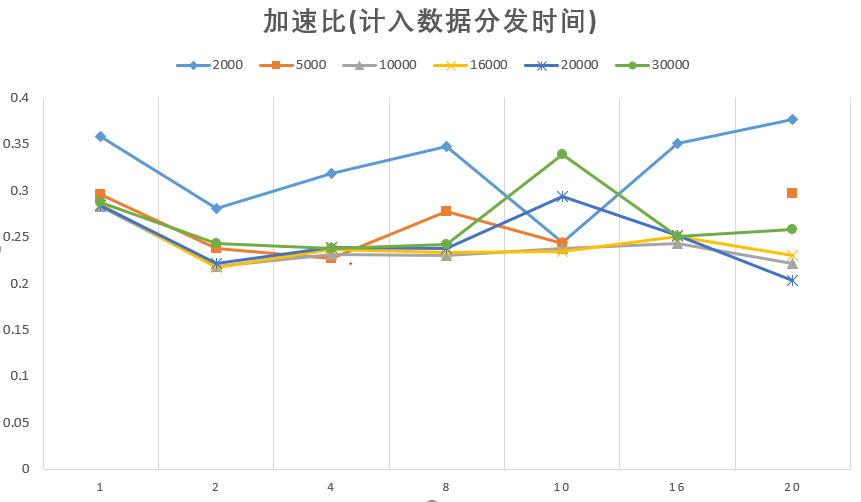
\includegraphics[width=0.8\textwidth]{hw3_1.png}
\end{figure}
\begin{figure}[htb]
	\centering
	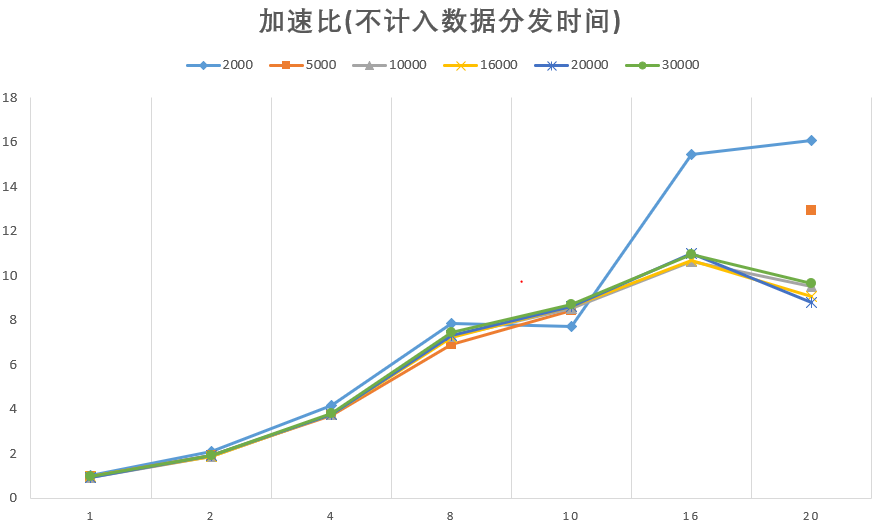
\includegraphics[width=0.8\textwidth]{hw3_2.png}
\end{figure}

\clearpage
\section{Exercise 3.6}
\subsection{运行方式}
\subparagraph*{}
./prog3\_6下放有makefile,在该目录下执行“\textbf{make}”可以得到可执行程序; 之后执行“\textbf{make run p=... n=...}”可以运行程序。其中p的值可以任选,如“\textbf{make run p=4 n=2000}”(默认p=16, n=100); 执行“\textbf{make clean}”可以删除生成的.o文件和可执行程序; 
\subparagraph*{}
注意: $p$应为完全平方数,且$n$应能被$\sqrt{p}$整除。
\subparagraph*{}
运行程序后,程序会随机生成一个$n\times n$的$double$矩阵和$n$维随机向量,分别采用的矩阵按块并行和串行策略计算$y = Ax$,统计并输出串行/并行运行时间、加速比、二范数误差等结果。
\subsection{代码思路}
\paragraph*{run\_submat():}
\subparagraph*{}
为了使得数据可以按分块矩阵进行数据分发,本函数使用MPI\_Cart\_create()定义了新的具有笛卡尔拓扑结构的通信子$comm$, 并使用MPI\_Cart\_sub()提取出某位置的通信子$row\_comm$, $col\_comm$, $diag\_comm$,分别负责分块矩阵的行、列和对角线的通信.
\begin{lstlisting}[language={c++}, title={定义新通信子}]
// Create a communicator of 2-dim Cart
MPI_Cart_create(MPI_COMM_WORLD, d, dims, periods, reorder, &comm);
// Build a communicator for each process row
free_coords[0] = 0, free_coords[1] = 1;
MPI_Cart_sub(comm, free_coords, &row_comm);
// Build a communicator for each process col
free_coords[0] = 1, free_coords[1] = 0;
MPI_Cart_sub(comm, free_coords, &col_comm);
// Get the group underlying comm
MPI_Comm_group(comm, &group);
// Create the new group
MPI_Group_incl(group, row_comm_sz, p_ranks, &diag_group);
// Create the communicator
MPI_Comm_create(comm, diag_group, &diag_comm);
\end{lstlisting}
\par 之后,我定义了新的派生数据类型$submat\_mpi\_t$,表示一个$\frac{n}{\sqrt{p}}\times\frac{n}{\sqrt{p}}$的矩阵块。
\begin{lstlisting}[language={c++}, title={定义派生数据类型}]
MPI_Datatype vect_mpi_t, submat_mpi_t;
MPI_Type_vector(loc_m, loc_n, n, MPI_DOUBLE, &vect_mpi_t);
MPI_Type_create_resized(vect_mpi_t, 0, loc_n * sizeof(double), &submat_mpi_t);
\end{lstlisting}
\par 进行数据分发:使用MPI\_Scatterv()函数将$matrix$中的元素按矩阵块分给各个进程。使用MPI\_Scatter()函数将$vector$的数据分给对角进程(diag)中的loc\_x[]($\frac{n}{\sqrt{p}}$维),对角进程在列内使用MPI\_Bcast()将分块向量分给同一列的进程的loc\_x[]。运算结束后,使用MPI\_Reduce()函数将每行的结果加总得到loc\_y[],保存在对角进程中。最后使用MPI\_Gather()函数将对角进程的结果收集到主进程。
\begin{lstlisting}[language={c++}, title={数据分发与收集}]
// Scatter data of matrix
MPI_Scatterv(matrix, counts, disp, submat_mpi_t, loc_A, loc_m * loc_n, MPI_DOUBLE, 0, comm);
// Scatter data of vector
MPI_Scatter(vector, loc_n, MPI_DOUBLE, loc_x, loc_n, MPI_DOUBLE, 0, diag_comm);
MPI_Bcast(loc_x, loc_n, MPI_DOUBLE, coords[1], col_comm);
// add up the partial sums in my process row and store the result on the diagonal
MPI_Reduce(sub_y, loc_y, loc_m, MPI_DOUBLE, MPI_SUM, coords[0], row_comm);
//gather data of results on the diagonal
MPI_Gather(loc_y, loc_n, MPI_DOUBLE, parallel_res, loc_n, MPI_DOUBLE, 0, diag_comm);
\end{lstlisting}
\begin{lstlisting}[language={c++}, title={计算}]
//matirx-vector multiply
for(int i = 0; i < loc_m; i++){
sub_y[i] = 0.0;
for(int j = 0; j < loc_n; j++){
sub_y[i] += loc_A[i * loc_n + j] * loc_x[j];
}
}
\end{lstlisting}
\subsection{测试结果}
下列样例运行“make run p=4 n=100”得到如下结果,可以看到,本例并行算法的二范数误差$error < 1e^{-10}$,达到了预期要求:
\begin{lstlisting}[language={}, title={$p=4, n=100$}]
[2018011446@bootstraper prog3_6]$ make run p=4 n=100
srun -n 4 -l ./matvectmul 100
0: error(2 norm):                                 0.00000000000000941541
0: time (Serial)                                  0.000021s
0: time (with MPI_Scatter/MPI_Reduce)             0.000435s
0: time (without MPI_Scatter/MPI_Reduce)          0.000006s
0: time (Scatter&Reduce)                          0.000429s
0: Speedup ratio(with MPI_Scatter/MPI_Reduce)     0.0487
0: Speedup ratio(without MPI_Scatter/MPI_Reduce)  3.3001
\end{lstlisting}
\subsection{性能评估}
下表展示了不同进程数$p$和矩阵大小$n$的性能测试结果:\\
运行时间及加速比的统计表与统计图如下:
\begin{table}[htb]
	\centering
	\begin{tabular}{l|llll}
		\hline
		$n \backslash p$& 1 & 4 & 16 & 25 \\ \hline
		2000 & 0.005/1.0439 & 0.002/2.3784 & 0.013/0.4618 & 0.168/0.0268 \\ \hline
		8000 & 0.073/0.9644 & 0.039/1.7993 & 0.190/0.3601 & 1.274/0.0311 \\ \hline
		12000 & 0.164/0.9612 & 0.068/1.7961 & 0.437/0.3506 & 2.234/0.0314 \\ \hline
		16000 & 0.264/0.9616 & 0.126/1.8334 & 0.768/0.3571 & 5.006/0.0315 \\ \hline
		24000 & 0.662/0.9636 & 0.188/2.2858 & 2.548/0.3496 & 8.891/0.0281 \\ \hline
		36000 & 1.485/0.9649 & \#N/A & \#N/A & \#N/A \\ \hline
	\end{tabular}
	\caption{Total time(s) \& Speedup Ratio(考虑数据分发)}
\end{table}
\begin{table}[htb]
	\centering
	\begin{tabular}{l|llll}
		\hline
		$n \backslash p$& 1 & 4 & 16 & 25 \\ \hline
		2000 & 0.005/1.0619 & 0.001/4.1508 & 0.0004/15.2852 & 0.0002/23.5762 \\ \hline
		8000 & 0.072/0.9665 & 0.018/3.7956 & 0.006/10.8752 & 0.001/21.1074 \\ \hline
		12000 & 0.163/0.9625 & 0.041/3.7985 & 0.014/10.7188 & 0.003/19.9999 \\ \hline
		16000 & 0.233/0.963 & 0.072/3.7988 & 0.022/12.1364 & 0.014/14.6549 \\ \hline
		24000 & 0.661/0.9641 & 0.315/3.7989 & 0.056/5.1244 & 0.015/17.3379 \\ \hline
		36000 & 1.484/0.9656 & \#N/A & \#N/A & \#N/A \\ \hline
	\end{tabular}
	\caption{Compute time(s) \& Speedup Ratio(不考虑数据分发)}
\end{table}
\begin{table}[htb]
	\centering
	\begin{tabular}{l|llll}
		\hline
		$n \backslash p$& 1 & 4 & 16 & 25 \\ \hline
		2000 & 0.0001 & 0.001 & 0.128 & 0.168 \\ \hline
		8000 & 0.0001 & 0.201 & 0.183 & 1.272 \\ \hline
		12000 & 0.0002 & 0.028 & 0.423 & 2.230 \\ \hline
		16000 & 0.0002 & 0.054 & 0.745 & 4.992 \\ \hline
		24000 & 0.003 & 0.075 & 2.491 & 8.877 \\ \hline
		36000 & 0.001 & \#N/A & \#N/A & \#N/A \\ \hline
	\end{tabular}
	\caption{Communication time(s)}
\end{table}
\begin{figure}[htb]
	\centering
	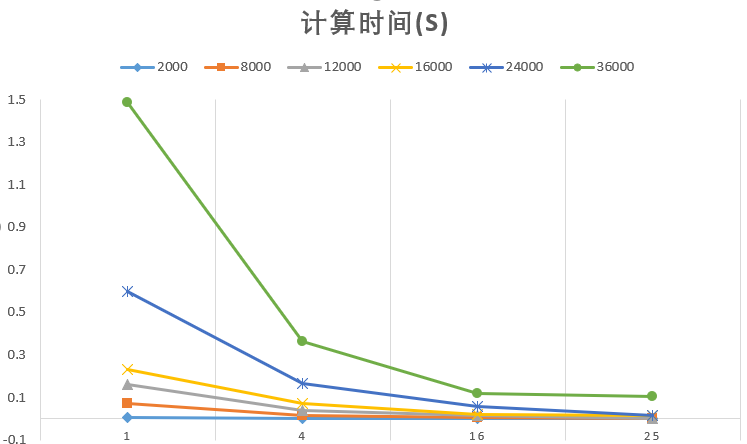
\includegraphics[width=0.8\textwidth]{hw3_6.png}
\end{figure}
\begin{figure}[htb]
	\centering
	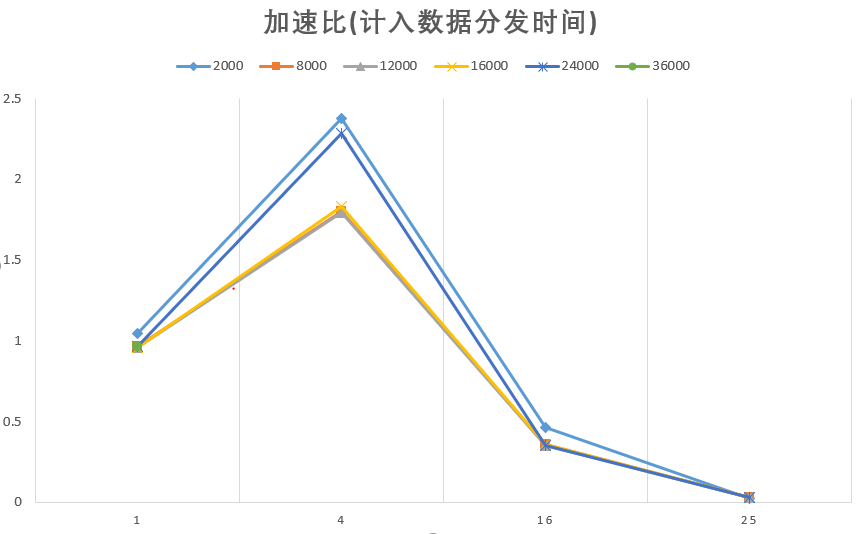
\includegraphics[width=0.8\textwidth]{hw3_3.png}
\end{figure}
\begin{figure}[htb]
	\centering
	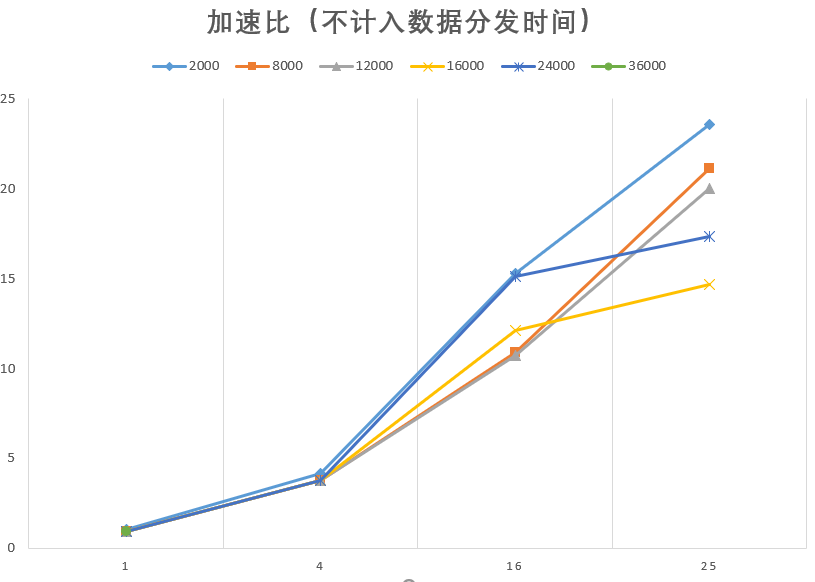
\includegraphics[width=0.8\textwidth]{hw3_4.png}
\end{figure}


\end{document}